%!TeX TS-program = lualatex
%!TeX encoding = UTF-8 Unicode
%!TeX spellcheck = en-UK
%!BIB TS-program = bibtex
% -*- coding: UTF-8; -*-
% vim: set fenc=utf-8
\documentclass{scrartcl}
\usepackage{fontspec}
\usepackage{geometry}
\geometry{a4paper, margin=1in}
\usepackage{hyperref}
\hypersetup{colorlinks=true, linkcolor=blue, urlcolor=blue}

% \usepackage[utf8]{inputenc}
\usepackage[T1]{fontenc}
\usepackage{amsmath}
\usepackage{amsfonts}
\usepackage{amssymb}
% \usepackage{siunitx}
% \sisetup{output-exponent-marker=\ensuremath{\mathrm{e}}}
% \newcommand{\ms}{\si{\milli\second}}%
\usepackage{graphicx}
\usepackage{tikz}
\usetikzlibrary{arrows.meta}
\usepackage{booktabs}
\usepackage{nicefrac}
\usepackage{microtype}
\usepackage{xcolor}
\usepackage{adjustbox}
\usepackage{dsfont}
\usepackage{url}
%
\usepackage[%
  square,        % for square brackets
  comma,         % use commas as separators
  numbers,       % for numerical citations;
%  sort,          % orders multiple citations into the sequence in which they appear in the list of references;
  sort&compress, % as sort but in addition multiple numerical citations
                 % are compressed if possible (as 3-6, 15);
]{natbib}
% In the bibliography, references have to be formatted as 1., 2., ... not [1], [2], ...
% \renewcommand{\bibnumfmt}[1]{#1.}
% \renewcommand{\bibsection}{\section*{References}} % requried for natbib to have "References" printed and as section*, not chapter*
%
%
\graphicspath{{../figures/}}

\title{
Working Memory with Polychronous Chains
}
\author{
  Laurent U Perrinet \\
  \texttt{laurent.perrinet@univ-amu.fr} \\
  Institut de Neurosciences de la Timone (UMR7289) \\
  Aix Marseille Univ, CNRS \\
  27 Bd Moulin, 13005 Marseille, France \\
  \url{https://laurentperrinet.github.io/publication/perrinet-26}
  % official institution "Aix Marseille Univ, CNRS, INT, Inst Neurosci Timone, Marseille, France" 
}
\date{\today}

\begin{document}
\maketitle

\begin{abstract}
Working memory --- the ability to store and recall precise temporal patterns of neural activity --- remains an open challenge for spiking neural networks (SNNs). We propose a recurrent SNN of $N=1024$ neurons in which each synapse is equipped with $D = 41$ heterogeneous delays, parameterised as a weight tensor $\mathbf{W} \in \mathbb{R}^{N \times N \times D}$ and trained end-to-end with surrogate-gradient backpropagation through time. Each stored pattern is represented as a sequential chain of overlapping Spiking Motifs: contiguous context windows of length $D$ that uniquely predict the activity at the next time step. A closed-form Hebbian initialisation, derived by deconvolving the LIF membrane response and targeting a sub-threshold membrane potential value superior to the threshold $\vartheta$, achieves an accuracy as measured by the $F_1$-score relative close to that expected when noise is present and before any gradient step on a benchmark of $M=16$ patterns of duration $T=1000\,\mathrm{ms}$. With learning, the network tolerates up to $25\%$ bit-flip noise, and reaches $F_1$ scrores closer to the value expected from the noise level. These results demonstrate attractor-like retrieval dynamics consistent with hippocampal pattern completion. These results show that heterogeneous synaptic delays are an efficient and scalable substrate for working memory in SNNs, with direct implications for neuromorphic edge deployment.
\end{abstract}
\noindent\textbf{Keywords:} Spiking Neural Networks, Polychronization; Heterogeneous delays, Working memory.

\section{Introduction}
%----------------------------%
% review biol cyb : The authors' strategy of subdividing a long motif into a series of shorter ones and then connecting a series of subnetworks to detect the long motif reminds this referee of the architecture of the original McCulloch-Pitts network (McCulloch, Warren S., and Walter Pitts. "A logical calculus of the ideas immanent in nervous activity." The bulletin of mathematical biophysics 5.4 (1943): 115-133.) Is there a natural way to interpret the authors' construction (which is in a continuous time neural network model) as a continuous time version of an analogous McCulloch-Pitts (hence, discrete time) model?
%----------------------------%
\begin{figure}%[t]
  % 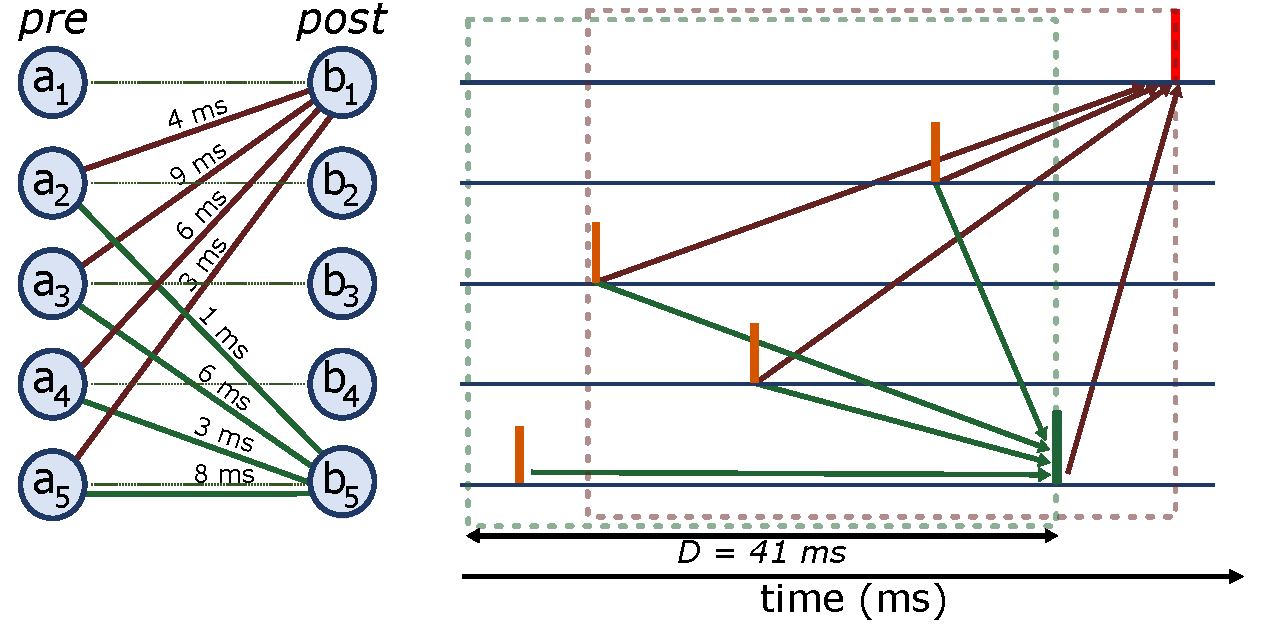
\includegraphics[width=\linewidth]{izhikevich_rec.pdf}%
  \begin{adjustbox}{width=\linewidth}
  \begin{tikzpicture}[
    x=1.2cm,
    y=1.2cm,
    >=Stealth,
    line cap=round,
    line join=round,
    font=\sffamily,
    neuron/.style={circle, draw=blue!70!black, line width=1.1pt, fill=blue!8, minimum size=1.05cm, inner sep=0pt},
    panelbox/.style={rounded corners=2pt, line width=1.1pt, dash pattern=on 2.2pt off 3.2pt},
    layer/.style={draw=blue!60!black, line width=1.2pt},
    brownlink/.style={draw=black!60!red!75!brown, line width=1.7pt},
    greenlink/.style={draw=green!40!black, line width=1.7pt},
    spike/.style={line width=3.3pt, draw=#1},
  ]
 
  \def\xLeftPanelLabel{-0.15}
  \def\xPostLabel{4.15}
  \def\xRightShift{7.4}
  \def\panelHeight{5.25}
  \def\spikeTop{4.95}
  \def\spikeBottom{0.14}
  \def\triggerBottom{0.18}
  \def\greenSpikeX{8.90}
  \def\greenSpikeFootY{0.18}
  \def\greenSpikeTopY{0.82}
  \def\redSpikeX{10.85}
  \def\redSpikeFootY{4.06}
  \def\redSpikeTopY{4.95}
  \def\spikeLift{0.56}
  \def\axisY{-0.85}
  \def\brownTargetY{\greenSpikeFootY}
  \def\greenTargetY{\redSpikeFootY}
  \pgfmathsetmacro{\brownTargetX}{\redSpikeX}
  \pgfmathsetmacro{\greenTargetX}{\greenSpikeX}
 
  % Orange trigger spikes parameters
  \def\oxOne{0.90} \def\oyFootOne{0.15} \def\oyTopOne{0.74}
  \def\oxTwo{2.95} \def\oyFootTwo{1.15} \def\oyTopTwo{1.98}
  \def\oxThree{4.85} \def\oyFootThree{2.02} \def\oyTopThree{2.83}
  \def\oxFour{7.95} \def\oyFootFour{3.02} \def\oyTopFour{3.84}
 
  % Left panel
  \node[anchor=south west, font=\itshape\Large] at (\xLeftPanelLabel,4.55) {pre};
  \node[anchor=south west, font=\itshape\Large] at (\xPostLabel,4.55) {post};
 
  \coordinate (a1) at (0,4);
  \coordinate (a2) at (0,3);
  \coordinate (a3) at (0,2);
  \coordinate (a4) at (0,1);
  \coordinate (a5) at (0,0);
 
  \coordinate (b1) at (4.55,4);
  \coordinate (b2) at (4.55,3);
  \coordinate (b3) at (4.55,2);
  \coordinate (b4) at (4.55,1);
  \coordinate (b5) at (4.55,0);
 
  \foreach \n in {1,...,5} {
    \draw[densely dotted, green!50!black] (a\n) -- (b\n);
  }
 
  \draw[brownlink] (a2) -- node[midway, sloped, above, fill=white, inner sep=1pt,
  font=\small] {4 ms} (b1);
  \draw[brownlink] (a3) -- node[midway, sloped, above, fill=white, inner sep=1pt,
  font=\small] {9 ms} (b1);
  \draw[brownlink] (a4) -- node[midway, sloped, above, fill=white, inner sep=1pt,
  font=\small] {6 ms} (b1);
  \draw[brownlink] (a5) -- node[midway, sloped, above, fill=white, inner sep=1pt,
  font=\small] {3 ms} (b1);
 
  \draw[greenlink] (a2) -- node[midway, sloped, below, fill=white, inner sep=1pt,
  font=\small] {1 ms} (b5);
  \draw[greenlink] (a3) -- node[midway, sloped, below, fill=white, inner sep=1pt,
  font=\small] {6 ms} (b5);
  \draw[greenlink] (a4) -- node[midway, sloped, below, fill=white, inner sep=1pt,
  font=\small] {3 ms} (b5);
  \draw[greenlink] (a5) -- node[midway, sloped, above, fill=white, inner sep=1pt,
  font=\small] {8 ms} (b5);
 
  \foreach \i/\p in {1/a1,2/a2,3/a3,4/a4,5/a5} {
    \node[neuron] at (\p) {$a_{\i}$};
  }
  \foreach \i/\p in {1/b1,2/b2,3/b3,4/b4,5/b5} {
    \node[neuron] at (\p) {$b_{\i}$};
  }
 
  % Right panel
  \begin{scope}[xshift=7.4cm]
    \coordinate (R0) at (0,0);
    \coordinate (R1) at (12.0,0);
    \coordinate (top) at (0,4.8);
 
    \draw[panelbox, draw=green!45!black, opacity=.35] (0.15,0.2) rectangle (10.15,
S4.8);
    \draw[panelbox, draw=black!35!red, opacity=.35] (2.0,0.2) rectangle (11.3,4.9)
;
 
    \foreach \y in {0,1,2,3,4} {
      \draw[layer] (0,\y) -- (11.8,\y);
    }
 
    % Orange trigger spikes
    \draw[orange!90!black, line width=3.5pt] (\oxOne,\oyFootOne) -- (\oxOne,\oyTopOne);
    \draw[orange!90!black, line width=3.5pt] (\oxTwo,\oyFootTwo) -- (\oxTwo,\oyTopTwo);
    \draw[orange!90!black, line width=3.5pt] (\oxThree,\oyFootThree) -- (\oxThree,\oyTopThree);
    \draw[orange!90!black, line width=3.5pt] (\oxFour,\oyFootFour) -- (\oxFour,\oyTopFour);
 
    % Green propagated spikes
    \draw[green!45!black, line width=3.5pt] (\greenSpikeX,\greenSpikeFootY) -- (\greenSpikeX,\greenSpikeTopY);
 
    % Red output spike
    \draw[red!90!black, line width=4.4pt] (\redSpikeX,\redSpikeFootY) -- (\redSpikeX,\redSpikeTopY);
 
    % Brown branches to the final spike (stems from foot)
    \draw[brownlink] (\oxOne,\oyFootOne) -- (\redSpikeX,4.65);
    \draw[brownlink] (\oxTwo,\oyFootTwo) -- (\redSpikeX,4.65);
    \draw[brownlink] (\oxThree,\oyFootThree) -- (\redSpikeX,4.65);
    \draw[brownlink] (\oxFour,\oyFootFour) -- (\redSpikeX,4.65);
 
    % Green branches converging on the lower output spike
    \draw[greenlink] (\oxOne,\oyFootOne) -- (\greenSpikeX,\greenSpikeFootY);
    \draw[greenlink] (\oxTwo,\oyFootTwo) -- (\greenSpikeX,\greenSpikeFootY);
    \draw[greenlink] (\oxThree,\oyFootThree) -- (\greenSpikeX,\greenSpikeFootY);
    \draw[greenlink] (\oxFour,\oyFootFour) -- (\greenSpikeX,\greenSpikeFootY);
    \draw[greenlink] (\greenSpikeX,\greenSpikeTopY) -- (\redSpikeX,4.35);
 
    % D marker and time axis
    \draw[<->, line width=1.1pt] (0.0,-0.16) -- node[below, font=\Large] {$D = 41\,\mathrm{ms}$} (\greenSpikeX,-0.16);
    \draw[->, line width=1.3pt] (0.0,-0.65) -- (12.4,-0.65) node[below, font=\Large] {time (ms)};
 
  \end{scope}
  \end{tikzpicture}
  \end{adjustbox}

  \caption{%
    \textbf{Working memory as a chained sequential spike prediction via heteroge
neous delays.}
    %
    \emph{Left:} A recurrent HD-SNN of five neurons numbered $1$--$5$, connected by two subsets of recurrent connections that define two Spiking Motifs from the pre-synaptic side (neurons $a$) to the post-synaptic side (neurons $b$): dark-r ed connections from $a_2$, $a_3$, $a_4$, and $a_5$ target $b_1$ with delays $4$, $9$, $6$, $3$\,ms; green connections from $a_1$, $a_2$, $a_3$, $a_4$ target $b_ 5$ with delays $1$, $6$, $3$, $8$\,ms. %
    \emph{Right:} Raster plot illustrating how the network predicts successive s pikes from a past context window.
    %
    \emph{Step~1 --- first prediction (green dashed box):} the orange input spik es emitted at staggered times by $a_2$--$a_5$ within the first context window (dashed green box) constitute a heterogeneous Spiking Motif. The green delays are tuned so that all four spikes converge \emph{synchronously} at $b_5$, crossing the firing threshold and producing the green output spike at a precise time. 
    %
    \emph{Step~2 --- second prediction (dark-red dashed box):} the green spike o f $a_5$ re-enters the network as a new input and, together with the spikes now visible in the shifted context window (dark-red dashed box), is routed through the dark-red delays in order to converge synchronously on $b_1$, generating a new output spike.
    %
    Because output spikes re-enter the same population, detecting one Spiking Motif provides the context for predicting the next spike in the sequence, implementing working memory as a chain of temporal predictions grounded in the preceding context window.
  }
  \label{fig:izhikevich}
\end{figure}

%----------------------------%
A century ago,~\citet{Adrian1926} established that neural communication relies on all-or-none action potentials, \emph{spikes}. Whether information is encoded in precise spike timing or in the coarser measure of instantaneous firing rate remains debated~\citep{Softky1993,Bohte2004,Grimaldi2023} --- a question that becomes especially sharp for working memory, where the brain must maintain and manipulate information across delays of seconds. In traditional artificial neural networks, long-range temporal dependencies are addressed by gated recurrent unit (GRU) architectures or Transformers~\citep{Vaswani2017}, which decouple temporal binding range from the timescale of individual units. The analogous problem for spiking neural networks (SNNs) --- binding activity patterns separated by intervals far exceeding a single neuron's time constant --- lacks a general solution and remains a key challenge for biologically plausible sequence processing~\citep{Yin2026}.

\citet{Izhikevich2006} extended the synfire framework by introducing heterogeneous axonal delays in a recurrent population of spiking neurons trained with spike-timing-dependent plasticity (STDP). The resulting \emph{polychronous neuronal groups} (PNGs) --- time-locked, non-synchronous firing patterns at millisecond precision --- vastly outnumber the neurons in the network, yielding a large short-term memory capacity exploited for visual feature binding~\citep{Eguchi2018} and sequence classification~\citep{Paugam-Moisy2008}.~\citet{Szatmary2010} showed that short-term plasticity can cue a PNG's reactivation and sustain a working memory. However, storing spike patterns of arbitrary length is inherently difficult: the sequential structure of the task means each context window is not an independent query but is itself the output of the network at the previous step, so small errors at early time steps propagate and amplify towards the end of the sequence --- a compounding difficulty absent from static associative memory like Hopfield networks.

The limitation of the original model from~\citet{Izhikevich2006} is that delays are fixed rather than learned. Recent work addresses this:~\citet{Goltz2021} demonstrated fast, energy-efficient inference on neuromorphic hardware using first-spike-time coding, while~\citet{Hammouamri2023} introduced gradient-based delay learning via dilated convolutions with learnable spacings (DCLS), achieving sparse solutions in which only $\sim\!20\%$ of delay channels remain active. Applied to event-based vision, heterogeneous learned delays in a single spiking layer suffice for fast motion detection~\citep{Grimaldi2023a}, scalable to always-on object recognition~\citep{Grimaldi2024}. Building on this, \emph{Spiking Motifs} (SMs) generalise PNGs to a gradient-trainable, hardware-compatible framework by replacing fixed STDP rules with end-to-end learned delays, here referred to as Heterogeneous-Delay SNNs (HD-SNNs)~\citep{Perrinet2023}. However these motifs have a short time span equal to the ranbge of possible delays, while it has been shown in mice stimulations that sequences of the order of seconds influence neural activity~\citep{Deveau2026}.~\citet{Kronland-Martinet2025} recently extended this to motifs of arbitrary length by chaining sub-motif detectors with bounded synaptic delays, achieving robust encoding of complete Spiking Heidelberg Digits patterns.

The present work extends the chain-of-motifs framework of~\citet{Kronland-Martinet2025} to a fully recurrent topology for working memory. Rather than relying on fixed delays and unsupervised STDP as in the original polychronisation model, the network is trained end-to-end with surrogate gradients~\citep{Neftci2019a}: once primed by a short trigger window of $D$ steps, it autonomously recalls arbitrary-length spike sequences, bridging polychronisation theory with gradient-based machine learning.

%%%-----------------------------------------------------------------
%%%-----------------------------------------------------------------
\section{Methods}
\label{sec:methods}
%%%-----------------------------------------------------------------
\subsection{Recurrent HD-SNN architecture} % MNESIS
%%%-----------------------------------------------------------------

In a previous work, we have demonstrated that a feedforward HD-SNN can learn to detect Spiking Motifs~\citep{Perrinet2023}. However, this architecture is limited to motifs of length $D$, the maximum synaptic delay. To store and recall longer sequences, it is possible to extend this architecture to a fully recurrent topology, where each neuron receives inputs from all other neurons across all delays. Our core concept is to retrieve a memory progressively, in which each motif of length $D$ would allow to predict the next spikes in the memory to retrieve. This allows the network to generate a chain of overlapping Spiking Motifs, where each motif provides the context for predicting the next spikes in the sequence (see Figure~\ref{fig:izhikevich}).

In practice, we will study a recurrent Heterogeneous-Delay SNN (HD-SNN) which consists of a population $\mathcal{A}$ of $N = 1024$ leaky integrate-and-fire (LIF) neurons implemented in \texttt{snnTorch}~\citep{Eshraghian2023} and simulated over $T = 1000$ steps of $1\,\mathrm{ms}$ each (total duration: $1\,\mathrm{s}$). Extending the feedforward Spiking Motif Detector~\citep{Perrinet2023}, our architecture will include full recurrence: each neuron $j \in \mathcal{A}$  integrates inputs from \emph{all} other neurons across \emph{all} preceding $D = 41$ time steps. Such network is the most general for learning purposes, and at inference, pruning of the synapses may be added to gain from the sparseness of synapses on the energy budget. Moreover, the choice for the maximum delay value $D$ is justified from biological observations and similar to the value used in the original polychronisation study~\citep{Izhikevich2006}. The membrane potential $u_j(t)$ evolves as
\begin{equation}
  u_j(t)
  = \beta \cdot u_j(t-1) \cdot (1 - s_j(t-1))
    + \sum_{i=1}^{N} \bigl (
      % b_i + 
      \sum_{d=1}^{D} \mathbf{W}_{j, i, d} \cdot s_i(t-d) \bigr ), 
  \label{eq:lif}
\end{equation}
where $\beta \in (0,1)$ is the membrane decay constant ($\beta = 0.8$ in our simulations, that is, a time constant of $\tau= 1 / \ln(\frac 1 \beta) \approx 4.5$ steps), $\mathbf{W}_{j, i, d}$ is the synaptic weight to neuron $j$ from neuron $i$ at delay $d$, and $s_j(t) \in \{0,1\}$  is the spike indicator $s_j(t) = \mathds{1}[u_j(t) \geq \vartheta]$, that is, $s_j(t)=0$ if $u_j(t) < \vartheta$ and a spike is emitted $s_j(t)=1$ when $u_j(t)$ exceeds the threshold $\vartheta$. After spiking, the membrane potential that is accumulated in Equation~\ref{eq:lif} is reset to zero.

In our implementation, the spike history of all $N$ neurons over the past $D$ steps is concatenated into a flattened context vector of dimension $N \cdot D$ at each time step, so that $\mathbf{W}$ is reshaped as $\mathbf{\bar W} \in \mathbb{R}^{N \times (N \cdot D)}$. This is equivalent to the temporal convolution that we used previously in a feedforward setting~\citep{Perrinet2023}, here extended to a fully recurrent topology. The HD-SNN thus maps onto a standard static computational graph that can be trained with surrogate gradient descent as classical SNNs (see Figure~\ref{fig:model}, left panel).

%%%-----------------------------------------------------------------
\subsection{Synthetic dataset}
%%%-----------------------------------------------------------------
To assess working-memory capacity in all generality, we generated a dataset of $M = 16$ distinct target patterns $\mathbf{S}^{(\mu)} \in \{0,1\}^{N \times T}$. Following previous work~\citep{Perrinet2023}, each pattern is generated using a stochastic spiking pattern generator with both a structured and background component. Specifically, for each pattern we define a \emph{frozen} pattern as $P^{(\mu)} \in \{0,1\}^{N \times T}$ with $
  P^{(\mu)} \sim \mathrm{Bernoulli}(p_A)$ 
where we set $p_A = 1.6 \times 10^{-4}$ spike per neuron per time step ($0.16\,\mathrm{Hz}$ if we consider $1\,\mathrm{ms}$ time bins) as the average spike probability. This follows the estimation of the average spiking frequency in the human brain~\citep{Lennie2003}. 

To account for the stochasticity inherent to neural activity, we further include a balanced bit flipping mechanism with probability $p_\text{flip} = 0.05$. This is defined by the binary mask  $M^{(\mu)} \in \{0,1\}^{N \times T}$ of bit flips locations :
$
  M^{(\mu)} \sim \mathrm{Bernoulli}(p_\text{flip})
  $.
Values are left untouched where $M^{(\mu)} = 0$ and will be drawn with probability $p_A$ where $M^{(\mu)} = 1$. Finally, the spike patterns $S^{(\mu)} \in \{0,1\}^{N \times T}$ are those of the frozen pattern $P^{(\mu)}$ except where $M^{(\mu)} = 1$ for which they are obtained by drawing with probability $p_A$. Formally, this can be expressed as:
\begin{equation}
  % \mathbf{S}^{(\mu)} \sim \mathrm{Bernoulli}(P^{(\mu)} \cdot (1 - M^{(\mu)}) + (1 - P^{(\mu)}) \cdot M^{(\mu)})
  \mathbf{S}^{(\mu)} \sim P^{(\mu)} \cdot (1 - M^{(\mu)}) + \mathrm{Bernoulli}(p_A) \cdot M^{(\mu)}
  \label{eq:pattern_generation}
\end{equation}
Note that the bit flipping mechanism introduces a stochasticity into the structure of the spike patterns, however, it does not change the average firing rate. Indeed, since the generation of $\mathbf{P}^{(\mu)}$ and $\mathbf{M}^{(\mu)}$ are independent, the expected firing rate $E(\mathbf{S}^{(\mu)})$ is equal to $p_A \cdot (1 - p_\text{flip}) + p_A \cdot p_\text{flip}= p_A$. 
%
%%%-----------------------------------------------------------------
\subsection{Working memory task: memory cuing}
%%%-----------------------------------------------------------------
%
Given a set of target patterns as defined above, a generic working memory task consists of training the network to reproduce the target pattern that follow a short \emph{trigger} window. Formally, given $\mathbf{S}^{(\mu)}$, each contiguous window of length $D$, i.e.\ the slice $\mathbf{S}^{(\mu)}[\cdot,\, t{-}D:t{-}1]$, constitutes a unique context that may be used to predict the spiking activity $s_j(t)$ of all neurons $j$ at time $t$ (see Figure~\ref{fig:izhikevich}). The network is therefore trained to generate a sequential chain of overlapping Spiking Motifs~\citep{Perrinet2023,Kronland-Martinet2025} that faithfully reproduces the target. Memory retrieval is cued by clamping all neuron activities to the target pattern during the trigger window which corresponds to the initial $D$ time steps ($0 \le t < D$), that is, corresponding to one elementary Spiking Motif (see Figure~\ref{fig:model}, right panel); the goal of the network is then to generate the remainder of the sequence autonomously.

As an accuracy metric, we will use the mean $F_1$ score between the predicted and target spike trains, averaged over time (in the prediction window), neurons and patterns. The $F_1$ score is the harmonic mean of precision (proportion of predicted activity that are correct) and recall (proportion of predicted activity that is successfully reproduced). Knowing a priori that average neural activity is sparse, maximising $\mathcal{L}$ simultaneously penalises over-active networks (low precision) and silent networks (low recall). 

Applied to the synthetic patterns, knowing $p_\text{flip}$ then one may first compute the precision as the ratio of expected true positives to the sum of true positives and false positives, that is, $\frac{p_A \cdot (1 - p_\text{flip} + p_A \cdot p_\text{flip})}{p_A \cdot (1 - p_\text{flip} + p_A \cdot p_\text{flip}) + p_\text{flip} \cdot (1 - p_A) \cdot p_A} = 1 - p_\text{flip} \cdot (1 - p_A)$. Then, recall is equal to precision as the average ratio of false negatives $p_A \cdot p_\text{flip}) + p_\text{flip} \cdot (1 - p_A) \cdot p_A$ is equal to that of false positives (remember that the average frequency is not changed by the balanced bit flip operation). As a result, the $F_1$ score between the frozen and perturbed patterns equals the precision and recall and is given by:
\begin{equation}
  F_1 = 1 - p_\text{flip} \cdot (1 - p_A)
  \label{eq:f1} 
\end{equation}
This will provide a theoretical bound for the average $F_1$ score that can be achieved by the network, as it is of course impossible to recover exactly the original frozen pattern (when $p_\text{flip}=0$) from a perturbed one  (when $p_\text{flip}>0$).

%%%-----------------------------------------------------------------
\subsection{Analytical weight initialisation}
%%%-----------------------------------------------------------------
\label{sec:init}
From Equation~\ref{eq:lif}, by normaizing the potential to arbitrary units, we wish the membrane potential to reach a sub-threshold value close to one whenever a spiking motif from a target pattern occurs. Before training, the weight tensor $\mathbf{W}$ can be initialised analytically by treating this task as a linear regression problem. For each target pattern $\mathbf{S}^{(\mu)} \in \{0,1\}^{N \times T}$, the context window at time $t$ is the flattened vector $\mathbf{c}^{(\mu)}(t) \in \{0,1\}^{N \cdot D}$ containing the spike history of all neurons over steps $t-D$ to $t-1$ and the corresponding desired output $\mathbf{I}(t) \in \{0,1\}^N$. Stacking all $K = M \cdot (T-D)$ context--output pairs across patterns and time steps yields
\[
  \mathbf{C} \in \{0,1\}^{(N \cdot D) \times K},
  \qquad
  \mathbf{I}^* \in \mathbb{R}^{N \times K},
\]
and the initialisation problem becomes $\mathbf{W}\,\mathbf{C} \approx \mathbf{I}$.

The choice of regression output $\mathbf{I}$ requires care. A naive choice is the binary spike matrix $\mathbf{S}$ itself, which would amount to ask the network to produce a current equal to the target spike at each step. However, the synaptic current $I_j(t) = \sum_{i,d} \mathbf{W}_{j,i,d} \cdot s_i(t-d)$ is not compared directly to $s(t)$: it is first \emph{filtered} by the membrane, which acts as a causal first-order IIR lowpass with transfer function $H(z) = 1/(1 - \beta \cdot z^{-1})$ and impulse response $h(t) = \beta^t$. The correct output is therefore obtained by deconvolution.  The inverse filter of $H(z)$ is $H^{-1}(z) = 1 - \beta \cdot z^{-1}$. Applied to a target trajectory that reaches $1$ at $t$ and resets immediately, the optimal input current is therefore
\begin{equation}
  I_j(t) \;=\; s_j(t) - \beta \cdot s_j(t-1).
  \label{eq:deconv_target}
\end{equation}
This is a \emph{biphasic} waveform: $1$ at each target spike time $t$ and $1-\beta$ exactly one step later, cancelling the residual membrane charge left by the leak. For $\beta \to 0$ the biphasic correction collapses to a scaled impulse; for $\beta = 0.8$ the negative lobe is substantial and significantly reduces spurious spikes.
 
Since the system is strongly underdetermined ($K \ll ND$), the minimum-$\ell_2$-norm solution is the Moore--Penrose pseudo-inverse $\mathbf{W}^* = \mathbf{I}^* \cdot \mathbf{C}^+$. With sparse neural activity at rate $p_A = .16\cdot 10^{-3}$, consecutive context windows are nearly orthogonal, so the Gram matrix satisfies $\mathbf{C}\mathbf{C}^\top \approx N \cdot D \cdot p_A \cdot \mathbf{I}$, giving the closed-form initialisation
\begin{equation}
  w_{i, j, d}
  = \frac{1}{N \cdot D \cdot p_A \cdot M}
    \sum_{\mu=1}^{M}\sum_{t=D+1}^{T}
    s_i^{*(\mu)}(t-d)
    \cdot
    \bigl(s_j^{*(\mu)}(t) - \beta \cdot s_j^{*(\mu)}(t-1)\bigr).
  \label{eq:init}
\end{equation}
Each weight $w_{i, j, d}$ is proportional to the cross-correlation between the deconvolved spike train of neuron $j$ (scaled by $\vartheta_0 = 0.8$) and the raw spike train of neuron $i$ at delay $d$, averaged over all $M$ patterns. 

 We will set the threshold at $\vartheta = 0.8$ at each target spike time $t$, reserving a safety margin $\delta = 1 - \vartheta = 0.2$. This margin prevents spurious firings from partial contexts and, crucially, places the membrane in the regime where the surrogate gradient is near its maximum, making the first gradient step maximally informative (see Appendix~\ref{app:margin} for the full derivation and its relationship to capacity)
 The $\vartheta_0$ factor ensures that a perfect context produces $u_j(t^*) = \vartheta_0$, leaving a margin $\delta = 0.2$ below the threshold. This mirrors spike-timing-dependent plasticity (STDP)~\citep{Izhikevich2006} and classical Hebbian learning~\citep{Perrinet2002}, with the additional $-\beta$ correction accounting for the membrane leak (full analysis in Appendix~\ref{app:margin}). At inference time the network receives its own generated context rather than the ground truth, so errors can accumulate over time --- the primary source of difficulty analysed in Section~\ref{sec:results}.
%%%-----------------------------------------------------------------
\subsection{Training}
%%%-----------------------------------------------------------------
%%%----------------------------------------------------------------- 
\begin{figure}%[htbp]
  \centering
  \adjustbox{valign=t,width=0.43\textwidth}{%
  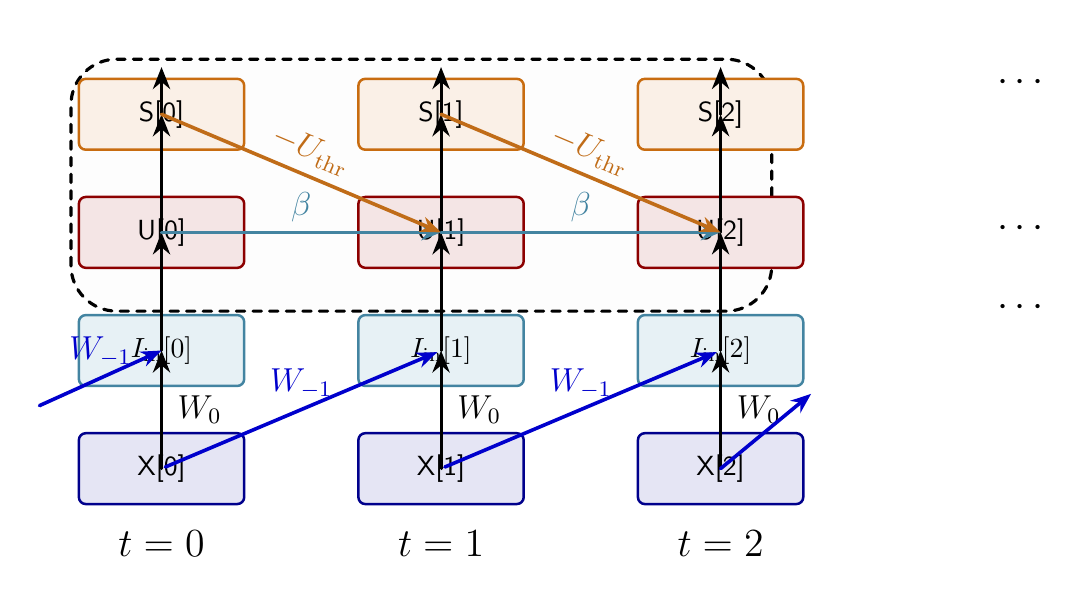
\begin{tikzpicture}[
    x=1cm,
    y=1cm,
    >=Stealth,
    line cap=round,
    line join=round,
    font=\sffamily,
    rect/.style={draw=#1, fill=#1!10, line width=0.9pt, rounded corners=2.5pt, minimum width=2.1cm, minimum height=0.9cm, inner sep=1pt},
    spike/.style={draw=black, line width=1.05pt, -{Stealth[length=2.8mm,width=2.2mm]}},
    beta/.style={draw=cyan!60!black, line width=1.2pt, -{Stealth[length=2.5mm,width=2.0mm]}},
    weights/.style={draw=blue!80!black, line width=1.3pt, -{Stealth[length=2.6mm,width=2.0mm]}},
    thr/.style={draw=orange!55!brown!85!black, line width=1.3pt, -{Stealth[length=2.6mm,width=2.0mm]}},
    labelbeta/.style={above, font=\large, text=cyan!60!black, midway},
    labelweights/.style={above, font=\large, text=blue!80!black, pos=0.50},
    labelthr/.style={above, sloped, font=\large, text=orange!55!brown!85!black, midway},
  ]
 
  \def\colSep{3.55}
  \def\xY{-2.05}
  \def\iY{-0.55}
  \def\uY{0.95}
  \def\sY{2.45}
  \newcommand{\colpos}[2]{({\colSep*#1,#2})}
  \def\tLabelY{-3.0}
  \def\ellipsisX{10.95}
  \def\blueRise{0.95}
  \def\blueRun{1.15}
 
  % Positions for the three time steps
  % (Removed manual coordinate definitions)
 
  % Dotted recurrent shell over U and S layers
  \path[draw=black, dashed, line width=1.15pt, rounded corners=0.58cm, fill=black!4, fill opacity=0.20] (-1.15,-0.05) rectangle (7.75,3.15);
 
  % Layer nodes
  \foreach \i in {0,1,2} {
    \node[rect=blue!55!black] at (\colSep*\i, \xY) {X[\i]};
    \node[rect=cyan!60!black] at (\colSep*\i, \iY) {$I_{\mathrm{in}}[\i]$};
    \node[rect=orange!70!brown!85!black] at (\colSep*\i, \sY) {S[\i]};
    \node[rect=red!55!black] at (\colSep*\i, \uY) {U[\i]};
  }
 
  % Vertical input chain
  \foreach \i in {0,1,2} {
    \draw[spike] (\colSep*\i, \xY) -- node[midway, right=2pt, font=\large] {$W_0$} (\colSep*\i, \iY);
    \draw[spike] (\colSep*\i, \iY) -- (\colSep*\i, \uY);
    \draw[spike] (\colSep*\i, \uY) -- (\colSep*\i, \sY);
    \draw[spike] (\colSep*\i, \sY) -- ++(0,0.6);
  }
 
  % Recurrent beta and threshold branches
  \foreach \i [evaluate=\i as \j using int(\i+1)] in {0,1} {
    \draw[beta] (\colSep*\i, \uY) -- node[labelbeta] {$\beta$} (\colSep*\j, \uY);
    \draw[thr] (\colSep*\i, \sY) -- node[labelthr] {$-U_{\mathrm{thr}}$} (\colSep*\j, \uY);
  }
 
  % Input weights between successive columns
  \draw[weights] (-1.55,-1.25) -- node[labelweights] {$W_{-1}$} (0, \iY);
  \draw[weights, shorten <=1.5pt, shorten >=1.5pt] (\colSep*0, \xY) -- node[labelweights] {$W_{-1}$} (\colSep*1, \iY);
  \draw[weights, shorten <=1.5pt, shorten >=1.5pt] (\colSep*1, \xY) -- node[labelweights] {$W_{-1}$} (\colSep*2, \iY);
  \draw[weights] (\colSep*2, \xY) -- ++(\blueRun,\blueRise);
 
  % Time labels
  \node[font=\Large] at (0,\tLabelY) {$t = 0$};
  \node[font=\Large] at (\colSep,\tLabelY) {$t = 1$};
  \node[font=\Large] at (2*\colSep,\tLabelY) {$t = 2$};
  \node[font=\Large] at (\ellipsisX,0.0) {$\cdots$};
  \node[font=\Large] at (\ellipsisX,1.0) {$\cdots$};
 
  % Top arrows and labels
  \node[font=\Large] at (\ellipsisX,2.85) {$\cdots$};
 
  % Clip-friendly top border for the dashed envelope
  \path[use as bounding box] (-1.7,-3.35) rectangle (9.8,3.55);
  \end{tikzpicture}%

  }
    \hfill
    \adjustbox{valign=t}{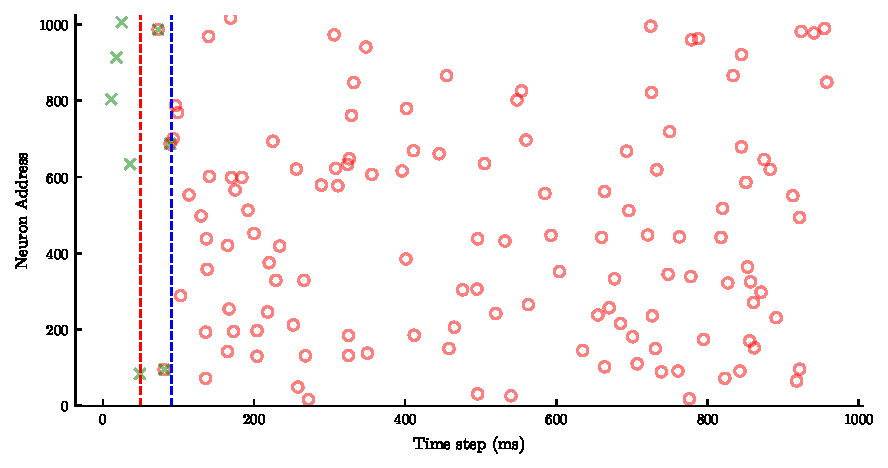
\includegraphics[width=0.52\textwidth]{pattern.pdf}}
  \caption{%
    Network architecture and a sample target pattern. \emph{Left:} Unrolled view of the recurrent HD-SNN over time (one column representing one time step), illustrating delayed connections between neurons: Blue arrows indicate synaptic connections that integrate past activity across heterogeneous delays; for clarity only one delay is shown. \emph{Right:} One representative target spike pattern ($N=1024$ neurons, $T=1000$ time steps, of which we show $256$ neurons and $400$ time steps); each red circle marks one target spike. The goal of the network is to memorise $M=16$ such patterns. Each trial is flanked by $N_\mathrm{pretime}=50$ time steps of spontaneous background activity (random spikes at rate $p_A$) before and after the stimulus. The trigger window (green crosses between the dashed lines) consists of the first $D=41$ time steps of the target pattern clamped to the network input; the recurrent network then autonomously predicts the remaining spikes.
  }\label{fig:model}
\end{figure}
%%%-----------------------------------------------------------------
The loss is defined as $\mathcal{L} = 1 - F_1$, such that minizing this loss (with a maximum of $1$ and minimum of $0$) maximises the mean $F_1$ score across all $M$ target patterns. Learning is carried out with surrogate-gradient BPTT~\citep{Neftci2019a}, using a fast-sigmoid surrogate with sharpness parameter $\alpha = 12$. Weights are optimised with SGD, using a cosine learning-rate schedule with warmup, as used for instance in~\citep{Hammouamri2023}, from a base learning rate $\eta_\mathrm{base} = 20.0 \times 10^{-3}$ to a final learning rate $\eta_\mathrm{final} = 400 \times 10^{-6}$, with $16$ warmup epochs over $256$ total epochs. Dropout regularization with probability $0.10$ is applied. The validation loss is monitored for detecting overfitting.

The gradient-based learning in our recurrent HD-SNN shares fundamental principles with biological STDP, despite operating at different scales. Both mechanisms exploit temporal correlations in spike timing to adjust synaptic strengths. However, while STDP implements local pairwise updates based on individual spike timings, our approach performs global optimisation that effectively learns the collective interaction of multiple delayed spike trains across the entire network. The analytical initialisation (see Equation~\ref{eq:init}) reveals this connection most clearly: it implements a Hebbian-like rule that is mathematically equivalent to averaging STDP updates across all stored patterns, suggesting that gradient descent in this context can be viewed as a principled, globally optimal implementation of temporally structured synaptic plasticity.

Our implementation is available at \url{https://github.com/laurentperrinet/MNESIS}. The recurrent HD-SNN was implemented using the snnTorch~\citep{Eshraghian2023} library with custom extensions for heterogeneous delay handling. The implementation leverages PyTorch with the Metal Performance Shader (MPS) backend for accelerated computation on Apple Silicon (M3 Ultra chip featuring 32 CPU cores and 80 GPU cores, with 512\,GB of unified memory architecture) and further tested with the CUDA backend on the Jean Zay supercluster at GENCI. The MPS and CUDA backends enabled efficient training and simulation of the large recurrent networks required for working memory tasks, leveraging the parallel processing capabilities of the GPU cores while maintaining low-latency access to the substantial memory resources necessary for storing all tensors' parameters. Training typically converged within $256$ gradient steps, requiring approximately $5$ minutes of computation time per training.
%
%%%----------------------------------------------------------------- 
\section{Results}
%%%----------------------------------------------------------------- 
\label{sec:results}
%%%----------------------------------------------------------------- 
\subsection{Training dynamics and results}
%%%----------------------------------------------------------------- 
%
Training the recurrent HD-SNN with surrogate-gradient BPTT~\citep{Neftci2019a} consistently maximised the mean $F_1$ score across all $M=16$ target patterns to approximately $0.9$, with $N=1024$ neurons, $D=41$ delays, $T=1000$ time steps, $p_A=1.6\times10^{-4}$, and $\beta=0.8$ (time constant $\tau \approx 4.5\,\mathrm{ms}$). Without the analytical initialisation, two characteristic failure modes arise during early training: episodes of complete silence, in which the network emits no spikes, and over-activation, in which nearly all neurons fire at every time step. Both are well-known pathological attractors of recurrent SNNs~\citep{Izhikevich2006}. The $F_1$ score is the harmonic mean of precision and recall, and maximising it therefore penalises both failure modes symmetrically: low precision corresponds to an over-active network and low recall to a silent one. The cosine learning-rate schedule~\citep{Hammouamri2023} helped guide the network away from these extremes towards a balanced, sparse-firing regime. 

Remarkably, the analytical weight initialisation alone (Eq.~\ref{eq:init}) already achieves high $F_1$ scores before any gradient step, demonstrating that the closed-form Hebbian solution provides a strong baseline for recall on this benchmark. The Gram-matrix approximation $\mathbf{C}\mathbf{C}^\top \approx N \cdot D \cdot p_A \cdot \mathbf{I}$ reduces the pseudo-inverse to a simple cross-correlation, yielding a ${\approx}5\times$ speed-up with identical accuracy; this approximation is used throughout. Gradient training serves primarily to improve robustness: errors arise when the trigger window is corrupted (Section~\ref{sec:robustness}), and learning helps mitigate their accumulation.

%%%----------------------------------------------------------------- 
\begin{figure}[!ht]
  \begin{center}
    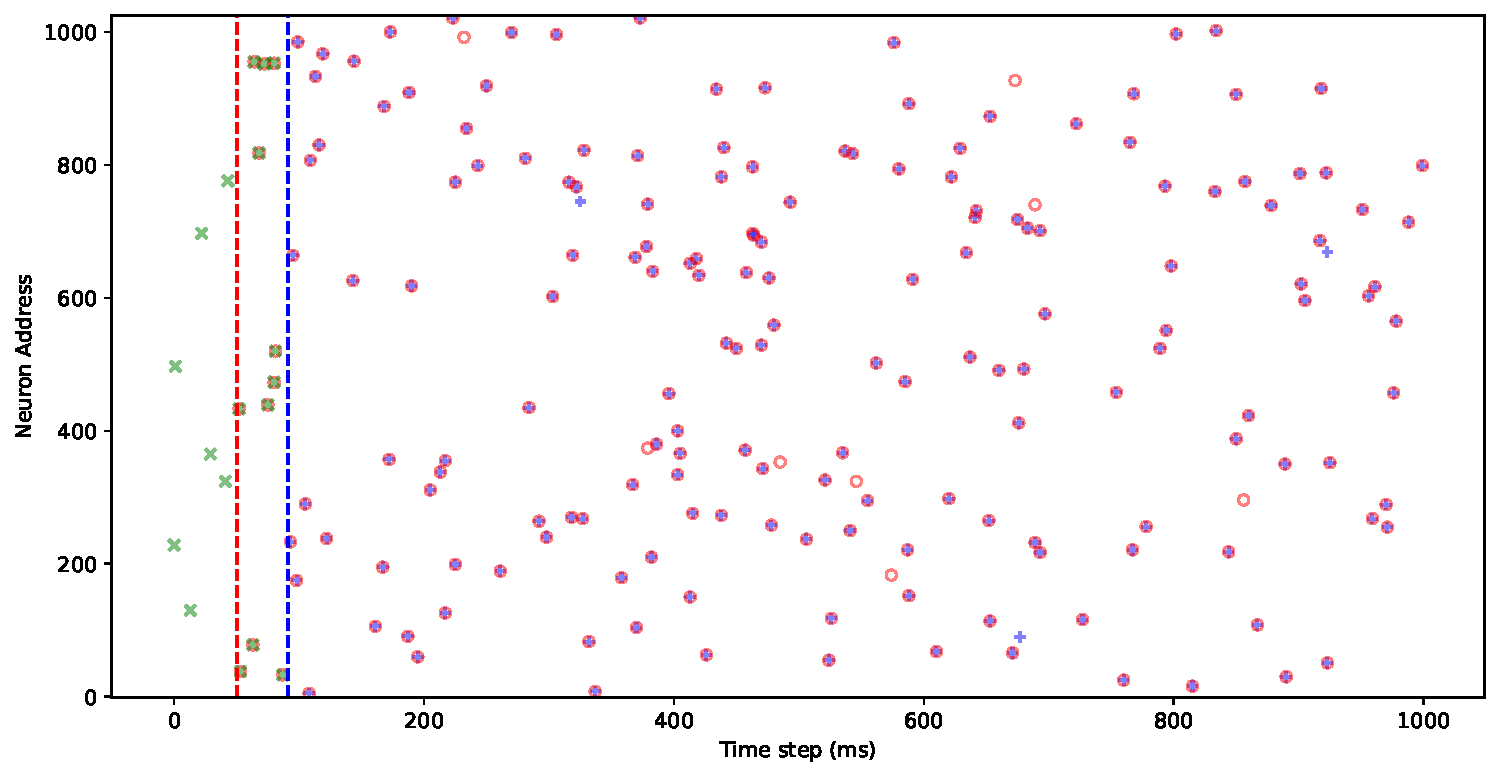
\includegraphics[width=\textwidth]{target.pdf}
  \end{center}
  \caption{Pattern retrieval from the recurrent HD-SNN. After clamping the network with input spikes (green crosses) with 50 steps of spontaneous activity (left of the red dashed line) and a trigger window consisting of the initial sequence of one of the $M=16$ target patterns ($0 \leq t < D = 41$, delimited by the dashed red and blue line), we simulate the network after training output the duration the full sequence duration ($T = 1000$ steps). We observe that the raster plot shows network activity (blue crosses, $N=1024$ neurons) which perfectly matches the target pattern which was cued during the trigger window. Note that the target spikes after the trigger window (red circles right of the blue dashed line) are hidden from the network.}\label{fig:target}
\end{figure}
%%%-----------------------------------------------------------------

%%%-----------------------------------------------------------------
\subsection{Effect of hyperparameters}
%%%-----------------------------------------------------------------
% 25_MNESIS_optuna.ipynb
We performed a systematic sweep over the key hyperparameters and report their effect on the mean $F_1$ score at convergence.

\paragraph{Surrogate sharpness $\alpha$.}
The sharpness of the surrogate gradient had the largest single effect on performance. Low values of $\alpha$ produced gradients that were too smooth to discriminate precise spike times, while excessively high values caused gradient vanishing. The default value used in this study is $\alpha = 12$, consistent with the robust training regime observed in our parameter scans.

\paragraph{Target firing rate.}
The best recall was obtained at low target firing rates (default $0.16\,\mathrm{Hz}$ per neuron), confirming that sparse activity facilitates stable recurrent dynamics~\citep{Izhikevich2006,Yin2026}. Higher firing rates led to increased inter-pattern interference and degraded precision, echoing the capacity bounds reported for polychronous neuronal groups~\citep{Szatmary2010}.

%%%-----------------------------------------------------------------
\subsection{Retrieval of multiple spike patterns}
%%%-----------------------------------------------------------------
%  this section reflects what is computed in 13_MNESIS_testing-inference.ipynb

Training was not uniform in time: the network first reproduced spikes immediately following the trigger window ($0 \leq t < D$), then progressively extended correct recall towards later time steps, as shown in Figure~\ref{fig:target}. This behaviour is a direct consequence of the sequential structure of the task: because each context window $[t-D,\, t-1]$ uniquely predicts the activity at time $t$, errors at early time steps propagate into all subsequent predictions, making temporal proximity to the trigger window the primary driver of learning progress.

To evaluate the network's ability to retrieve and distinguish multiple stored patterns in sequence, we concatenated all $M=16$ patterns into a single long raster, each trial flanked by $N_\mathrm{pretime}=50$ steps of spontaneous background activity at rate $p_A$ before and after the stimulus (Figure~\ref{fig:retrieval}). Each pattern was triggered by its individual trigger window, and retrieval was evaluated by a sliding-window $F_1$ score over time. The $F_1$ score rose sharply at the onset of each trigger window, remained high throughout each pattern's duration, and dropped back to the background level during the inter-trial intervals, confirming that the network correctly associates each trigger window with its corresponding stored pattern without cross-interference between the $M=16$ stored memories.

%%%----------------------------------------------------------------- 
\begin{figure}[!ht]
\begin{center}
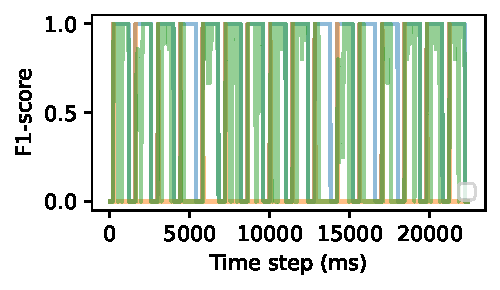
\includegraphics[width=\textwidth]{retrieval.pdf}
\end{center}
\caption{Sequential retrieval of the $M=16$ stored patterns. The sliding-window $F_1$ score (blue) is shown as a function of time, together with the onset indicator of each trigger window (green dashes) and the corresponding pattern mask (red dashes). The $F_1$ score rises sharply at each trigger-window onset and remains high for the full pattern duration ($T=1000$ steps $\sim 1$ second), then returns to baseline during the inter-trial intervals, demonstrating selective retrieval of all stored memories in sequence without cross-interference.}\label{fig:retrieval}
\end{figure}
%%%-----------------------------------------------------------------

%%%-----------------------------------------------------------------
\subsection{Working memory and robustness to perturbations}
\label{sec:robustness}
%%%-----------------------------------------------------------------
%
A hallmark of biological working memory is graceful degradation: recall should remain possible under incomplete or corrupted retrieval cues, mirroring the tolerance of hippocampal pattern completion to partial input~\citep{Villette2015}. We therefore evaluated three distinct perturbations of the trigger window, each probing a different dimension of robustness (Figure~\ref{fig:noise}).

\paragraph{Robustness to spike noise (Figure~\ref{fig:noise}, left).}
% 14_MNESIS_testing-noise.ipynb
We corrupted the trigger window by independently flipping each spike with probability $p_\mathrm{flip} \in [0, 1]$ (bit-flip noise). At $p_\mathrm{flip} = 0.25$, the network still achieved an $F_1$ score of $\approx 0.627$ (precision $\approx 0.898$, recall $\approx 0.481$), demonstrating a reasonable tolerance to noise in the trigger window. The $F_1$ score decreases monotonically as $p_\mathrm{flip}$ increases, reaching chance level only near $p_\mathrm{flip} = 0.5$ where the trigger window is entirely randomised. This behaviour is consistent with the network operating as an attractor: small perturbations of the initial state are corrected by the recurrent dynamics, which converge back to the stored pattern.

\paragraph{Robustness to trigger-window duration (Figure~\ref{fig:noise}, middle).}
% 15_MNESIS_testing-trigger-duration.ipynb
We varied the duration of the trigger window from $0$ to $D-1 = 40$ steps, scanning from no cue at all to a trigger that is one step short of the full motif. At $75\%$ of the full trigger duration ($\approx 30$ steps out of $D = 41$), the network achieved an $F_1$ score of $\approx 0.416$ (precision $\approx 0.632$, recall $\approx 0.310$). The $F_1$ score increases monotonically with trigger duration, rising steeply once the trigger exceeds roughly $D/2$, consistent with the requirement that the context window must contain enough active synapses to uniquely identify the stored pattern above the interference floor.

\paragraph{Robustness to partial neuron coverage (Figure~\ref{fig:noise}, right).}
% 16_MNESIS_testing-trigger-fraction.ipynb
We varied the number of neurons whose activity was silenced during the trigger window, from $0$ (full trigger) to $N = 1024$ (no trigger). With $N/8 = 128$ neurons silenced --- meaning $87.5\%$ of the population remained active --- the network still achieved an $F_1$ score of $\approx 0.602$ (precision $\approx 0.837$, recall $\approx 0.469$). The $F_1$ score degrades smoothly as more neurons are silenced and drops sharply only when the majority of the trigger population is inactive, again consistent with an attractor interpretation in which a sufficient fraction of the pattern suffices to pull the network dynamics towards the stored memory.
%
%%%----------------------------------------------------------------- 
\begin{figure}[!t]
\centering
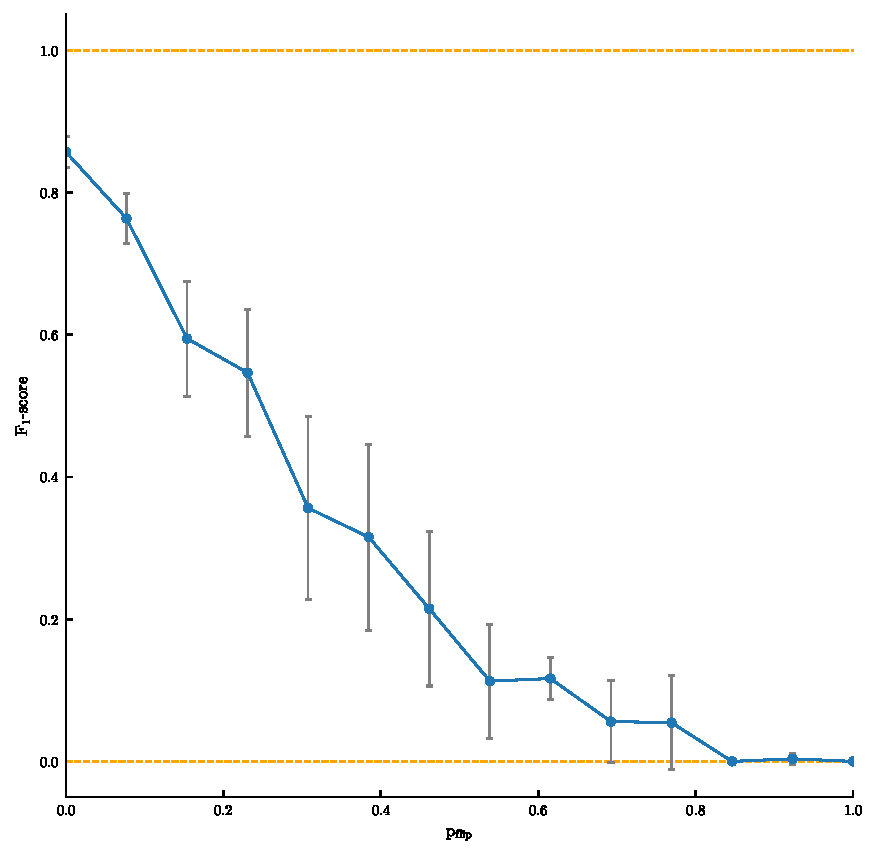
\includegraphics[width=0.325\linewidth]{p_flip_score.pdf}\hfill
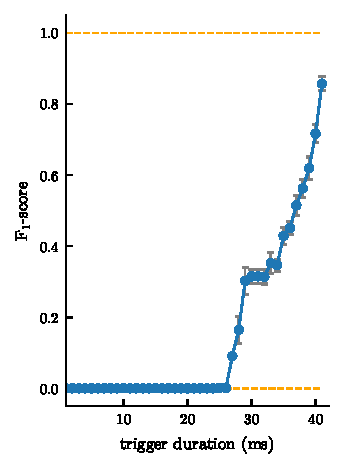
\includegraphics[width=0.325\linewidth]{trigger_time_score.pdf}\hfill
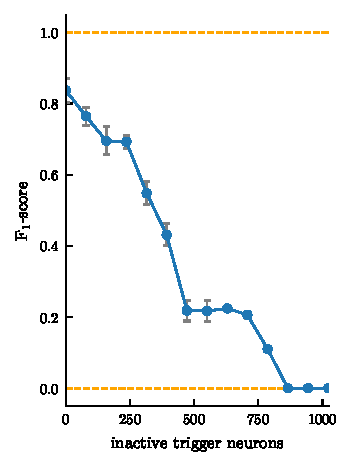
\includegraphics[width=0.325\linewidth]{fraction_target_score.pdf}
\caption{Robustness of working-memory retrieval to three types of trigger-window perturbation ($F_1$ score averaged over $M=16$ patterns). \emph{Left:} Bit-flip noise applied to all spikes in the trigger window ($p_\mathrm{flip} \in [0,1]$); the network maintains high $F_1$ up to $p_\mathrm{flip} \approx 0.4$. \emph{Middle:} Truncated trigger window (trigger duration from $0$ to $D-1 = 40$ steps); retrieval remains reliable for durations above roughly $D/2$. \emph{Right:} Partial neuron coverage (number of silenced neurons from $0$ to $N = 1024$); perfect recall is maintained until the majority of the trigger population is inactive. Orange dashed lines indicate $F_1 \in \{0, 1\}$.}\label{fig:noise}
\end{figure}
%%%-----------------------------------------------------------------
%
%%%-----------------------------------------------------------------
\subsection{Effect of delay depth, pattern duration, and background firing rate}
%%%-----------------------------------------------------------------
%  20_MNESIS_scanning-parameters.ipynb

To characterise how the architectural parameters govern working-memory performance, we conducted a systematic one-at-a-time scan over the maximum delay $D$, the pattern duration $T$, and the background firing rate $p_A$, holding all other hyperparameters at their default values (Section~\ref{sec:methods}). Each condition was evaluated with $N_\mathrm{cv} = 10$ independent random seeds and results are reported as mean loss $\mathcal{L} = 1 - F_1$ (Figure~\ref{fig:scan}).

\paragraph{Delay depth $D$ (Figure~\ref{fig:scan}, left).}
The loss decreases monotonically as $D$ grows from $3$ to $127\,\mathrm{ms}$, dropping from $\mathcal{L} \approx 0.85$ at $D = 3$ to near zero at $D = 127$. This confirms the capacity argument: the parameter budget $N^2 \cdot D$ and the context-window size $N \cdot D$ both scale linearly with $D$. A wider delay window provides more temporally diverse synaptic pathways, increasing the number of simultaneously representable Spiking Motifs and reducing interference between overlapping context windows. At $D = 3$ the context vector has only $N \cdot D = 3072$ dimensions with expected activity $N \cdot D \cdot p_A \approx 3.07$ --- a regime where contexts are nearly all-zero and indistinguishable. At $D = 127$ the context has $N \cdot D = 129{,}024$ dimensions with expected activity $\approx 129$, and near-orthogonality is strongly satisfied.

%%%----------------------------------------------------------------- 
\begin{figure}[!t] 
  \centering
  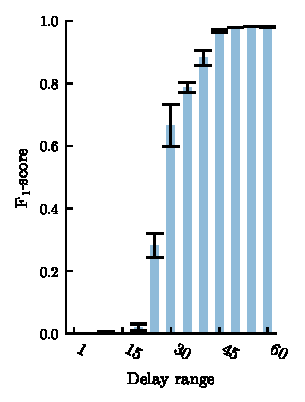
\includegraphics[width=0.6\linewidth]{scan_num_delay.pdf}\hfill
  % TODO 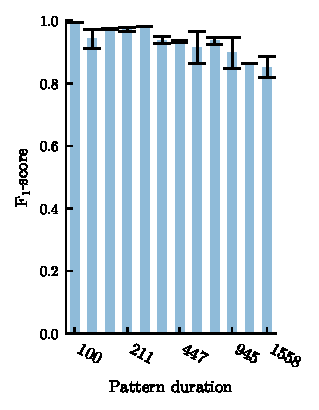
\includegraphics[width=0.6\linewidth]{scan_N_time.pdf}\hfill
  % TODO 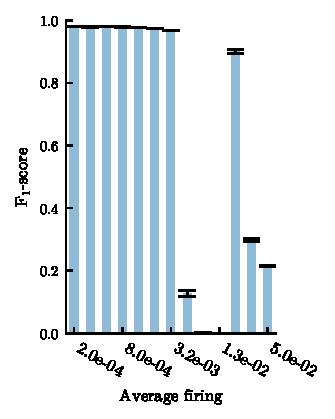
\includegraphics[width=0.9\linewidth]{scan_p_A.pdf}
  \caption{%
    Effect of some key parameters on working-memory performance (loss $\mathcal{L} = 1 - F_1$, mean $\pm$ s.e.\ over $N_\mathrm{cv} = 10$ cross-validation folds). %
    \emph{Left:} Increasing the maximum delay $D$ consistently reduces the loss, confirming that deeper delay windows provide a larger, more orthogonal context and that longer maximum delays directly increase the capacity of the recurrent HD-SNN. % (Section~\ref{sec:capacity}). %
    \emph{Right:} 
    % \emph{Middle:} 
    Loss grows slowly and monotonically with pattern duration $T$, consistent with the compounding-error and gradient-vanishing arguments: longer sequences require the network to maintain coherent predictions further from the trigger window. %
    % Performance is optimal at low background firing rates ($p_A \lesssim 10^{-3}$) and degrades sharply at higher rates. 
  }\label{fig:scan}
\end{figure}
%%%----------------------------------------------------------------- 
\paragraph{Pattern duration $T$ (Figure~\ref{fig:scan}, middle).}
The loss grows monotonically with $T$, from $\mathcal{L} \approx 0.004$ at $T = 64$ to $\mathcal{L} \approx 0.08$ at $T = 2048$. This is the empirical signature of the two compounding difficulties identified in the capacity analysis: longer sequences impose a larger open-loop rollout, and the error propagation recurrence accumulates over $T - D$ steps. Even a sub-critical propagation coefficient $\lambda < 1/D$ eventually allows errors to reach a non-negligible fraction of $N$ spikes.

% \paragraph{Background firing rate $p_A$ (Figure~\ref{fig:scan}, right).}
% The loss exhibits a clear optimum around $p_A = 10^{-4}$ to $10^{-3}$ and degrades rapidly for $p_A \geq 2 \times 10^{-3}$. Increasing $p_A$ linearly reduces the SNR of the cross-correlation initialisation and increases the Gram-matrix off-diagonal terms, degrading context orthogonality.

Taken together, the  scans quantitatively validate the theoretical framework: delay depth is the primary capacity lever (loss $\propto 1/(N \cdot D \cdot p_A)$), pattern duration is the primary difficulty lever, and firing rate sets the orthogonality regime that determines whether initialisation and learning converge. These results suggest that the most efficient path to storing longer patterns is to increase $D$ rather than $N$, since $D$ enters both the parameter capacity $N^2 \cdot D$ and the context orthogonality $N \cdot D \cdot p_A$ while adding no new neurons or lateral connections. Increasing $D$ is, however, ultimately limited by biological constraints on axonal conduction delays~\citep{Grimaldi2023a}.

% ICANN
%%%-----------------------------------------------------------------
% \subsection{Retrieval of periodic spike patterns}
%%%-----------------------------------------------------------------
%  this section reflects what is computed in 30_MNESIS_learn-periodic.ipynb

% %%%-----------------------------------------------------------------
% \subsection{Retrieval of traveling wave patterns}
% %%%-----------------------------------------------------------------
%  this section reflects what is computed in 32_MNESIS_learn-travelling-waves.ipynb



%%%----------------------------------------------------------------- 
\section{Discussion}
%%%-----------------------------------------------------------------

\subsection{Memory capacity and the role of heterogeneous delays}
%%%-----------------------------------------------------------------

We have demonstrated that a recurrent SNN with heterogeneous synaptic delays can store and reproduce arbitrary target spike patterns, with the analytical weight initialisation providing a strong starting point for recall on a benchmark of $M=16$ patterns of $T=1000$ steps. The result is noteworthy from a capacity standpoint: the entire network is parameterised by a single weight tensor $\mathbf{W} \in \mathbb{R}^{N \times N \times D}$ of dimension $N^2 \cdot D = 1024^2 \cdot 41 \approx 43 \times 10^6$ parameters, yet it faithfully stores $M$ patterns each of $N \cdot T$ binary values. This compression is made possible precisely by the temporal structure introduced by the $D$ delay channels: rather than requiring one parameter per stored bit, the network exploits the sequential dependencies between consecutive context windows of length $D$ to represent the entire pattern as a chain of overlapping Spiking Motifs~\citep{Perrinet2023,Kronland-Martinet2025}. The memory limit is determined by parameter count rather than interference --- the marginal parameter cost per additional stored pattern is zero, and the capacity scales as $N^2 \cdot D$, linear in the delay depth. This provides concrete evidence that heterogeneous delays are a computational asset rather than a biological nuisance, a point argued theoretically in~\citet{Izhikevich2006} and demonstrated empirically in the context of learnable delays in feedforward~\citep{Grimaldi2023a,Hammouamri2023} and recurrent architectures~\citep{Queant2025,Meszaros2025}, and which we extend here to a full working-memory setting.

% TODO importance of sparse coding~\citep{Perrinet2002image}

The robustness experiments further strengthen this interpretation. The network tolerates up to 25\% bit-flip noise in the trigger window, requires only $75\%$ of the full trigger duration for reliable recall, and maintains perfect retrieval with up to $87.5\%$ of trigger neurons silenced. This progressive degradation profile is consistent with the network operating as an attractor: the stored patterns correspond to stable fixed points of the recurrent dynamics, and the trigger window provides a partial cue that the network completes autonomously --- the same mechanism proposed for hippocampal pattern completion~\citep{Villette2015}.

\subsection{Limitations and directions for improvement}
%%%-----------------------------------------------------------------

The present model is deliberately minimal, and several design choices impose limits on capacity and robustness that future work should address.

\paragraph{Capacity and scaling.}
A systematic evaluation of memory capacity --- how many patterns of what duration can be reliably stored and retrieved --- remains to be carried out beyond the present $M=16$ benchmark. The theoretical analysis predicts that capacity scales as $N^2 \cdot D / (T-D)$, giving approximately $5{,}700$ patterns for the current architecture, but whether gradient-based training reliably reaches this bound at scale is an open empirical question, as the implementation does not scale well with respect to the size of the GPU's memory. Interference between stored patterns at high memory load may degrade precision in ways that the F1 training objective does not fully penalise, and the sensitivity of recall to perturbations of the trigger window is expected to decrease as $M$ grows.

\paragraph{Richer neuron models and dynamics.}
We used the simplest LIF model with a fixed membrane decay $\beta$. Introducing adaptive threshold dynamics or more complex single-neuron models, as studied in~\citet{Szatmary2010}, should increase the diversity of intrinsic timescales available to the network and improve both capacity and retrieval fidelity. In particular, the deconvolution analysis (Section~\ref{sec:methods}) shows that the optimal weight profile depends critically on $\beta$: larger values of $\beta$ require exponentially amplified weights at long delays, suggesting that adaptive $\beta$ per neuron could allow the network to exploit the full delay range more efficiently.

\paragraph{Latent reservoir neurons.}
The current architecture connects every neuron directly to every other neuron across all delays. Partitioning the population into input-output neurons and a larger pool of latent ``reservoir'' neurons, as in delay-based reservoir computing~\citep{Paugam-Moisy2008}, would enrich the internal spiking dynamics without increasing the number of trained parameters proportionally. Such a hybrid architecture could combine the representational power of random recurrent networks with the precision of gradient-trained delay weights~\citep{Neftci2019a}, potentially closing the gap between biologically inspired models and sparse selective-update architectures~\citep{Yin2026}. It is also possible to integrate the concept of chunking in a hierarchical architecture~\citep{Zhong2026}, where the recurrent HD-SNN serves as a high-level controller that orchestrates the activation of multiple parallel reservoirs, each specialised for different temporal scales or pattern types.

\paragraph{Online and unsupervised learning.}
% TODO introduce other learning types see \citep{Koopman2026}
The present model requires a fixed set of target patterns known in advance. A natural extension is an online learning rule that updates the weights continuously as new patterns are presented, without catastrophic forgetting of previously stored sequences. The closed-form Hebbian initialisation (Eq.~\ref{eq:init}) suggests a natural online update: each new spike $s_j(t)$ incrementally adjusts $w_{i, j, d}$ in proportion to $s_i(t-d)$, recovering a local STDP-like rule~\citep{Izhikevich2006}. Whether such online updates are stable under recurrent feedback and can support continual working memory remains to be established.

\subsection{Perspectives: unsupervised learning and neural data}
%%%-----------------------------------------------------------------

The most immediate application of this framework is to neurophysiological data. The supervised memorisation task studied here requires a known target pattern, but in practice one would like to discover the latent Spiking Motifs present in recorded multi-unit activity --- the problem originally addressed by~\citet{Ikegaya2004} and~\citet{Villette2015}. A natural extension is to replace the supervised F1 loss with a self-supervised or contrastive objective that trains the network to predict upcoming spikes from the recent spike history, without access to ground-truth labels. This is analogous to the contrastive predictive coding paradigm applied to continuous neural time series, here instantiated in a fully spike-based setting~\citep{Grimaldi2023}. Such a model would provide a principled, energy-efficient method for identifying the temporal structure of neural population codes, with direct relevance to the debate on rate coding versus temporal coding~\citep{Softky1993,Bohte2004} and to understanding the neural mechanisms of working memory more broadly. Deployed on neuromorphic hardware~\citep{Goltz2021,Eshraghian2023}, it could operate in real time on streaming electrophysiological data, opening a new avenue for closed-loop brain-machine interface applications.
%
%%%----------------------------------------------------------------- 
%%%----------------------------------------------------------------- 
\section*{Acknowledgements}
\noindent 
This work was performed using HPC resources from GENCI-IDRIS (Grant 2025--AD010314955R2).
The authors declare no competing interests regarding this manuscript. The funders had no role in the design of the study; in the collection, analyses, or interpretation of data; in the writing of the manuscript; or in the decision to publish the results.
For the purpose of open access, the authors have applied a CC-BY public copyright licence to any Author-Accepted Manuscript version arising from this submission, and the different versions are available on arXiv at \url{https://arxiv.org/abs/2604.14096}.
\section*{Statement on the use/non-use of Generative Artificial Intelligence}
\noindent 
In the preparation of this paper, the Gemma4:31b generative AI tool (provided through \url{https://ollama.com/library/gemma4:31b-mlx})
was used in a limited capacity. Its use was confined to language editing, namely improving the clarity, grammar, and phrasing of text  already drafted, as well as occasional technical assistance during the development of code. Generative AI was not used to generate research ideas, formulate the research questions or hypotheses, design the methodology, conduct or interpret any data analysis, or perform any mathematical derivations or calculations. All intellectual contributions, analytical work, and mathematical reasoning in this thesis are my own. I have reviewed all AI-assisted material and take full responsibility for the entire content of this thesis, including its accuracy and integrity.
%%%----------------------------------------------------------------- 
% ICANN suppression
\appendix
%%%----------------------------------------------------------------- 


%%%-----------------------------------------------------------------
\subsection{Representation of spiking activity}
%%%-----------------------------------------------------------------

In neurobiological recordings or the output of event-based cameras, any generic raster plot consists of a stream of \emph{spikes}, defined as a list of address--timestamp tuples to form an address-event representation (AER)~\citep{Grimaldi2024}. Formally, we define the event stream as
\[
  \mathcal{E}
  = \bigl\{(a_r,\, t_r)\bigr\}_{r \in [1,\, N_\mathrm{ev}]},
\]
where $N_\mathrm{ev} \in \mathbb{N}$ is the total number of events and $r$ indexes each event in the natural temporal order~\citep{Grimaldi2024}. Each event has a time of occurrence $t_r$ and an address $a_r$ in the neural population space $\mathcal{A}$. In a Single Unit Activity (SUA) recording for instance, $\mathcal{A}$ is the identified set of neurons.

Neurons are characterised by their membrane potential dynamics and by the integration of synaptic potentials along their dendritic tree. Crucially, neurons can receive inputs from multiple pre-synaptic neurons with \emph{heterogeneous delays} $\delta_s$, representing the travel time from the spike generation in the pre-synaptic neuron to its arrival at the soma of the post-synaptic neuron. Scanning all pre- and post-synaptic pairs, we define the set of $N_s \in \mathbb{N}$ synapses as
\[
  \mathcal{S}
  = \bigl\{(a_s,\, b_s,\, w_s,\, \delta_s)\bigr\}_{s \in [1,\, N_s]},
\]
where $a_s \in \mathcal{A}$ and $b_s \in \mathcal{A}$ are respectively the pre- and post-synaptic addresses, $w_s$ is the synaptic weight, and $\delta_s$ is the delay. Note that neurons in the human cortex have on average 30000 synapses~\citep{Rockland2002}, an order of magnitude which is seldom reached in artificial networks. In our model, two neurons may contact each other via multiple synapses, each with a different delay. The \emph{receptive field} of neuron $b$ is the sub-set of synapses that project onto it:
\[
  \mathcal{S}^b
  = \bigl\{(a_s,\, b_s,\, w_s,\, \delta_s) \mid b_s = b
    \bigr\}_{s \in [1,\, N_s]}.
\]
Each spike from the event stream $\mathcal{E}$ gets multiplexed in time by these synapses to later converge on the post-synaptic neurons.
%  into a new stream
% \[
%   \bigcup_{r=1}^{N_\mathrm{ev}}
%   \bigl\{(b_s,\; w_s,\; t_r + \delta_s)\bigr\}_{s \in \mathcal{S}_{a_r}},
% \]
% which in biology is naturally ordered in time as spikes arrive at post-synaptic somas. 
Crucially, as they reach  the post-synaptic neuron, a synchronous convergence of multiple spikes on the soma --- made possible by the interplay of heterogeneous delays --- increases the post-synaptic firing probability, enabling the detection of precise spiking motifs (see Figure~\ref{fig:izhikevich}).

To allow for the simulation of this network on standard hardware we transform this event-based representation into the Boolean matrix $A \in \{0,1\}^{N \times T}$, where $N = |\mathcal{A}|$ is the number of neurons and $T$ is the number of discrete time steps of $1\,\mathrm{ms}$ each (see Figure~\ref{fig:model}, right panel). Delays are discretised as integers in $[1, D]$, so the synaptic set for all neurons is compactly represented by
% The full connectivity is encoded in the 
the weight tensor
$\mathbf{W} \in \mathbb{R}^{N \times N \times D}$, with
% which corresponds to
% the kernel matrix $K^b$ of Section~\ref{sec:methods}.1 for every neuron
% $b$ simultaneously.
% the kernel matrix
% $K \in \mathbb{R}^{N \times N \times D}$, with
\[
  \mathbf{W}_{b_s, a_s, \delta_s} = w_s
  \quad \forall s \in [1,\, N_s],
  \quad \text{and zero otherwise.}
\]


\section{Sub-threshold initialisation target, surrogate gradient sensitivity, and capacity}
\label{app:margin}

\subsection{Surrogate gradient sensitivity}

The weight initialisation (Eq.~\ref{eq:init}) is designed so that a perfect context $\mathbf{c}(t) = \mathbf{c}^*(t)$ produces $u_j(t^*) = \vartheta_0 = 0.8$, strictly below the firing threshold $\vartheta = 1$. The safety margin $\delta = 0.2$ has two complementary justifications.

\paragraph{Surrogate gradient sensitivity.}
With the fast-sigmoid surrogate $\sigma_\alpha(x) = 1/(1 + |\alpha x|)^2$ at sharpness $\alpha = 12$, the gradient at the initialised membrane value $u_j(t^*) - \vartheta = \vartheta_0 - \vartheta = -0.2$ is
\[
\sigma_{12}'(-0.2) = \frac{12}{(1 + 12 \times 0.2)^2} \approx 1.04,
\]
remaining of order unity. Had $\vartheta_0 \ll \vartheta$, the gradient would be near zero and the first training steps would carry no useful signal. The choice $\vartheta_0 = 0.8$ therefore places the initialised network in a high-sensitivity regime.

\paragraph{Protection against spurious spikes.}
At inference time the network receives its own generated context $\hat{\mathbf{c}}(t)$. The resulting membrane perturbation has zero mean and standard deviation
\[
\sigma_u \approx \vartheta_0 \cdot \sqrt{\frac{p_A}{N \cdot D}} \approx 0.8 \times \sqrt{\frac{1.6\times10^{-4}}{1024 \times 41}} \approx 4.9 \times 10^{-5}.
\]
The probability of a spurious spike is $\Phi(-\delta/\sigma_u) = \Phi(-4048) \approx 0$, so the margin $\delta = 0.2$ provides essentially complete protection against spurious firings from random context errors. Any value $\delta \gtrsim 0.01$ would suffice; the larger value $0.2$ is chosen to maximise the gradient sensitivity argument above.

\subsection{Relationship to capacity}

The parameter-count capacity is
\[
M^* = \frac{N^2 \cdot D}{T - D} = \frac{1024^2 \times 41}{959} \approx 44{,}830 \text{ patterns.}
\]
A secondary, interference-limited capacity arises from the condition $\delta > \sigma_u \cdot \sqrt{M}$, giving
\begin{equation}
M^*_\delta = \frac{\delta^2 \cdot N \cdot D}{\vartheta_0^2 \cdot p_A} = \frac{(0.2)^2 \times 1024 \times 41}{(0.8)^2 \times 1.6\times10^{-4}} \approx 16{,}400{,}000.
\label{eq:M_cap_delta}
\end{equation}
Since $M^*_\delta \gg M^*$, the binding constraint is always the parameter count, not interference. The margin $\delta$ does not limit capacity; it governs only the quality of the gradient signal at initialisation.

%%%%%%%%%%%%%%%%%%%%%%%%%%%%%%%%%%%%%%%%%%%%%%%%%%%%%%%%%%%%
\bibliographystyle{plainnat}
\bibliography{mnesis}
% \printbibliography
%%%%%%%%%%%%%%%%%%%%%%%%%%%%%%%%%%%%%%%%%%%%%%%%%%%%%%%%%%%%
\end{document}
